% F092｜高中数学常用数值表｜03_proof.tex
% 继承上传模板的 LaTeX 环境；当前条目的内容独立编写。
\clearpage
\begin{proofbox}
\textbf{\textcolor{CProof}{核对方法一：用平方还原根号}}
\par\medskip
\begin{center}
% F092｜square 原创简明教学示意图
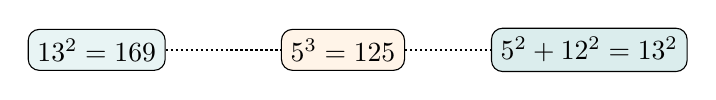
\begin{tikzpicture}[>=stealth,scale=.92]
\node[draw,rounded corners,fill=teal!9] (a) at (0,0){$13^2=169$};
\node[draw,rounded corners,fill=orange!9] (b) at (3.4,0){$5^3=125$};
\node[draw,rounded corners,fill=teal!14] (c) at (6.8,0){$5^2+12^2=13^2$};
\draw[densely dotted,thick] (a)--(b);\draw[densely dotted,thick] (b)--(c);
\end{tikzpicture}

\end{center}
\medskip
$1.414^2=1.999396$，接近 $2$；$2.236^2=4.999696$，接近 $5$。这能快速\textbf{检查}根号值，但不能把“接近”当作严格证明。若要控制误差，参见 F086。
\end{proofbox}
\clearpage
\begin{proofbox}
\textbf{\textcolor{CProof}{核对方法二：用对数运算联系多个数}}
\par\medskip
\begin{center}
% F092｜derive 原创简明教学示意图
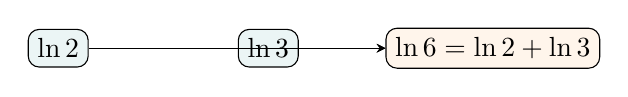
\begin{tikzpicture}[>=stealth,scale=.92]
\node[draw,rounded corners,fill=teal!8] (a) at (0,0){$\ln2$};
\node[draw,rounded corners,fill=teal!8] (b) at (2.9,0){$\ln3$};
\node[draw,rounded corners,fill=orange!8] (c) at (6,0){$\ln6=\ln2+\ln3$};
\draw[->] (a)--(c);\draw[->] (b)--(c);
\end{tikzpicture}

\end{center}
\medskip
利用 $\ln(ab)=\ln a+\ln b$，得到 $\ln6=\ln2+\ln3$。利用 $\lg10=1$ 得 $\lg5=1-\lg2\approx0.699$。这些是\textbf{关系证明}，不是三位小数本身的精确推导。
\end{proofbox}
\clearpage
\begin{proofbox}
\textbf{\textcolor{CProof}{核对方法三：平方与勾股数关系}}
\par\medskip
\begin{center}
% F092｜square 原创简明教学示意图
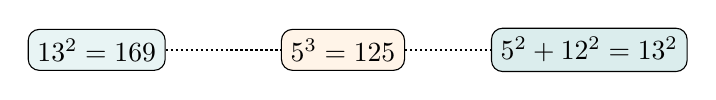
\begin{tikzpicture}[>=stealth,scale=.92]
\node[draw,rounded corners,fill=teal!9] (a) at (0,0){$13^2=169$};
\node[draw,rounded corners,fill=orange!9] (b) at (3.4,0){$5^3=125$};
\node[draw,rounded corners,fill=teal!14] (c) at (6.8,0){$5^2+12^2=13^2$};
\draw[densely dotted,thick] (a)--(b);\draw[densely dotted,thick] (b)--(c);
\end{tikzpicture}

\end{center}
\medskip
$13^2=169=5^2+12^2$，$25^2=625=7^2+24^2$。以平方表互相验证勾股数组，在做计算题时能减少查错成本。
\end{proofbox}
